\documentclass[12pt]{article}
\usepackage[margin=1in]{geometry}
\usepackage{hyperref}
\usepackage{graphicx}
\usepackage{subcaption}
\graphicspath{ {../images/} }

\begin{document}
	\title{\textbf{Object Detection}\\
		\small{CS725: Project Proposal}}
	\author{
			Pratik Kalshetti (163050048) \hfill 
			Ashish Jaiswal (163050055)\\
			Naman Rastogi (163050056) \hfill
			Prafull Gangawane (163050080)	}
	\date{}
	\maketitle
	
	\section*{Project Description}
	The aim of this project is to implement a system which is capable of detecting objects in a scene. The input to this system will be an image and the output will be a bounding box around the object along with the class label of the corresponding object. This box will be defined by 4 real numbers; x and y coordinate of the centre of the box, height and width of the box. The output class label will have a score associated with it, which denotes the confidence of the class prediction.
	
	This problem can be formulated as a regression problem for estimating the bounding box and a classification problem for predicting the class. Thus this project serves as a platform to develop a system based on the concepts of classification and regression which are the main contents of the course syllabus.
	
	The goal is to achieve accurate object detection at a high speed. 
	
	\begin{figure}[h]
		\centering
		\begin{subfigure}	[h]{0.4\textwidth}
			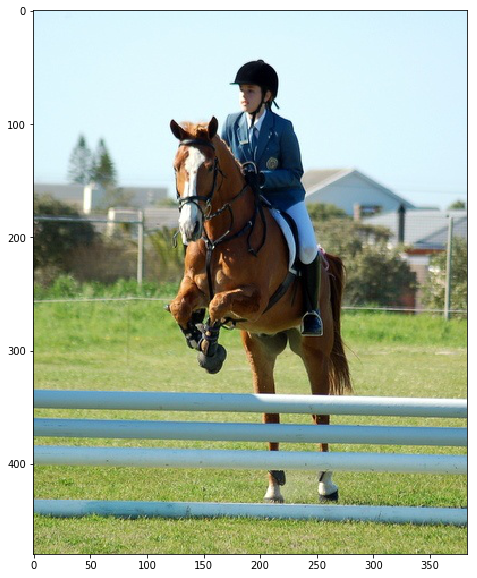
\includegraphics[width=\textwidth]{input.png}
			\subcaption{Input}
		\end{subfigure}
		\hfill
		\begin{subfigure}	[h]{0.4\textwidth}
			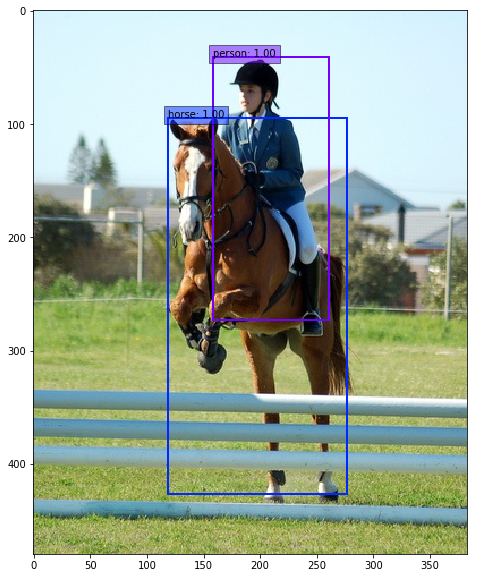
\includegraphics[width=\textwidth]{output.png}
			\subcaption{Output}
		\end{subfigure}
		\caption{System Specification}
	\end{figure}
		
	\section*{Approach}
	\paragraph{Background}
	The most successful methods in object detection consist of two major approaches -  two step detection \cite{girshick14CVPR, girshickICCV15fastrcnn, renNIPS15fasterrcnn}, and unified approach \cite{Redmon_2016_CVPR, liu2016ssd}. The two step detection strategy produces accurate results, however it lacks the performance speed which is tackled by a unified approach. Also this approach achieves the goals (accuracy and speed) of this project. 
	
	\paragraph{Details}
	The plan is to implement  an end-to-end deep neural network based on the ideas of \cite{liu2016ssd}. The task of feature extraction from the images will be achieved by using a pre-trained network on ImageNet data	\cite{imagenet_cvpr09} and then fine tune the network for the detection task. The deep network will be a fully convolutional network (FCN). The advantage of using a FCN is that any input image size is allowed. Also the spatial information is preserved by these kinds of networks for images and they tend to be computationally efficient when compared to fully connected layers.  The initial layers will help detect smaller objects, while the later layers will be useful for bigger objects. The output from some of these layers will be passed onto specialized networks which will work as classifier and localizer. Finally a non-maximum suppression  algorithm will be applied to filter the multiple boxes per object based on their confidence in prediction.  During training the error function to minimize consists of a combined classification and regression loss. 
	
	A more ambitious plan is to generate a new data set of different objects  and test the network for evaluating cross-dataset performance. Another intention is to detect objects in videos for real-time object detection.
	
	\section*{Research Papers}
	The ideas in \cite{liu2016ssd} will help in implementing the network. This paper introduces Single Shot Multibox Detector (SSD) which is the algorithm used in the standard API for object detection in tensorflow, thus proving its impact. 
	
	\section*{Dataset}
	For the purpose of this project, the publicly available PASCAL VOC dataset will be used. It consists of $10$k annotated images with $20$ object classes with $25$k object annotations. These images are downloaded from flickr. This dataset is used in the PASCAL VOC Challenge which runs every year since 2006.  
	
	
	\begin{figure}[h]
		\centering
			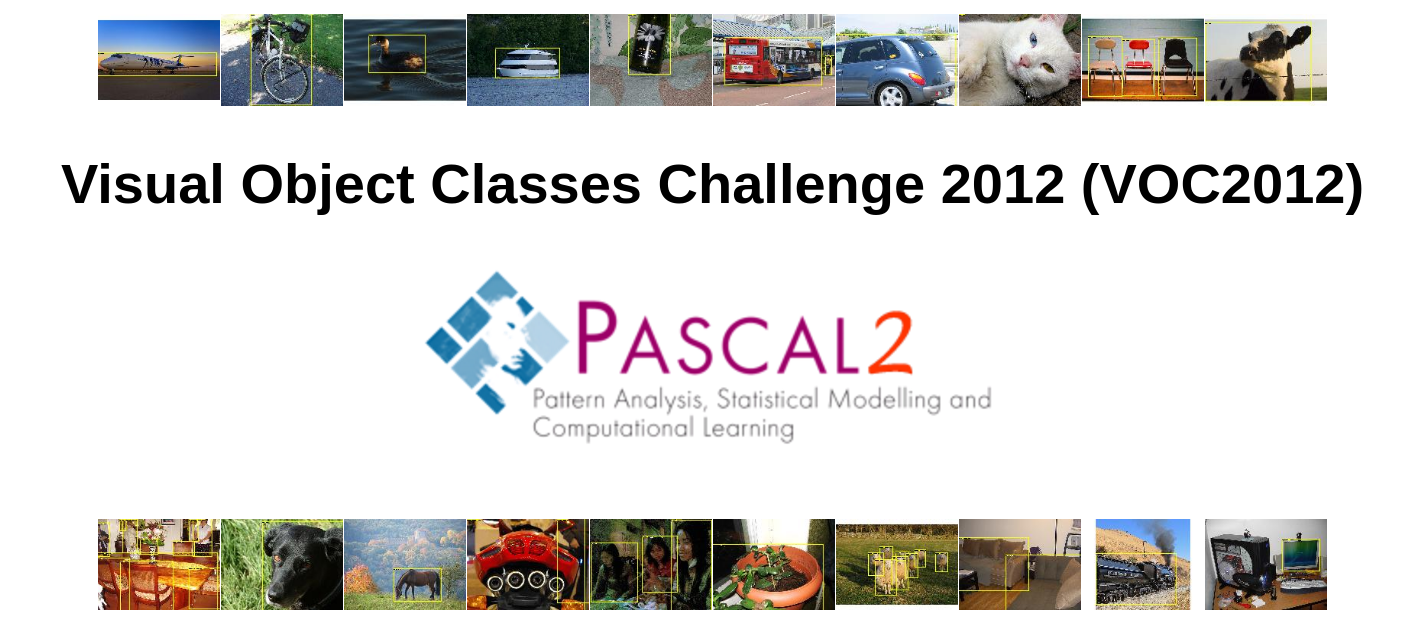
\includegraphics[height=1in]{dataset.png}
		\caption{Dataset}
	\end{figure}
	
	\bibliographystyle{unsrt}
	\bibliography{references}
	
\end{document}